\chapter{Hands-On: DDD Sample Application}
\section{Import der DDD Applikation in die IDE}
\begin{longtable}{| p{5cm} | p{11cm} |}
\hline
Die Vorlage Applikation kann in Eclipse als bestehendes Maven Projek importiert werden.
&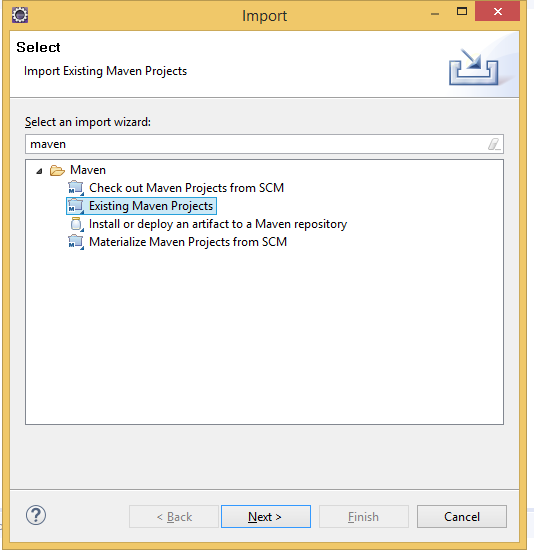
\includegraphics[width=0.65\columnwidth, valign=T]{images/ddd_basic/1.png}
 \\ \hline
Im Projektverzeichnis die pom.xml Datei auswählen.
&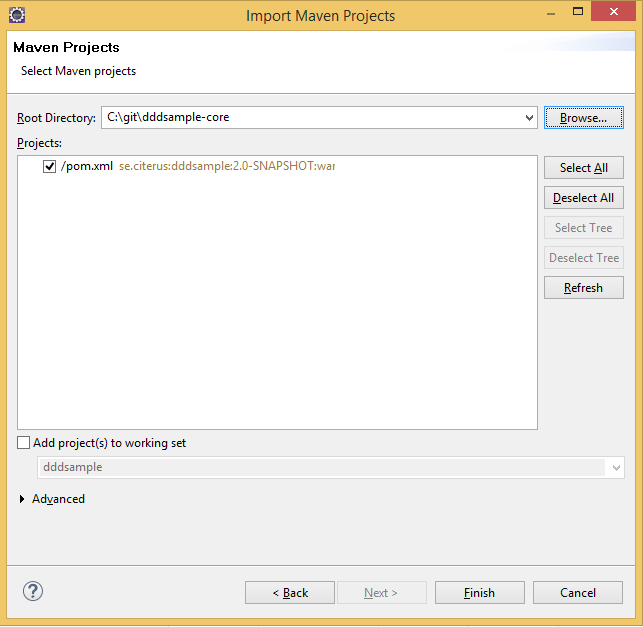
\includegraphics[width=0.65\columnwidth, valign=T]{images/ddd_basic/2.png}
 \\ \hline
Die Swisscom PaaS Cloud arbeitet mit Cloud Foundry. Das Cloud Foundry Plugin für Eclipse kann über den MarketPlace installiert werden.
&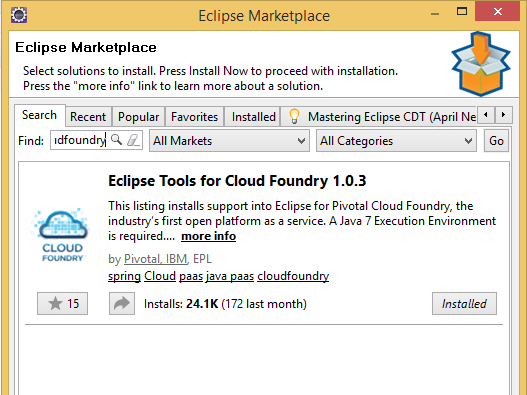
\includegraphics[width=0.65\columnwidth, valign=T]{images/ddd_basic/3.png}
 \\ \hline 
Nun müssen die Maven Dependencies geladen werden.
&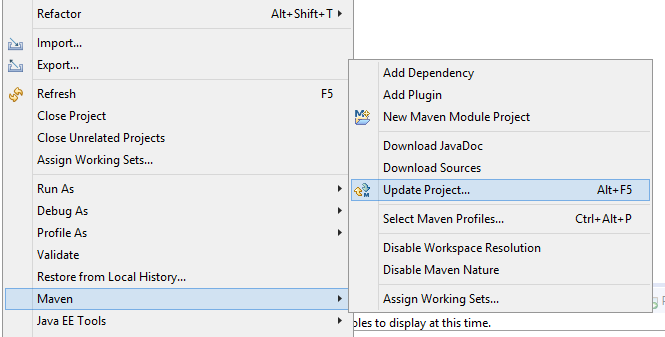
\includegraphics[width=0.65\columnwidth, valign=T]{images/ddd_basic/4.png}
 \\ \hline
Jetzt kann der Build-Prozess gestartet werden.
&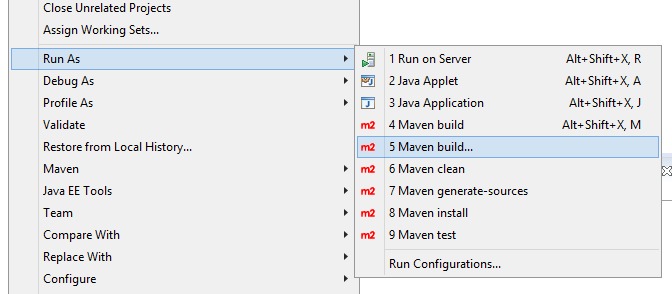
\includegraphics[width=0.65\columnwidth, valign=T]{images/ddd_basic/5.png}
\\ \hline 
\end{longtable}
\newpage
\section{Deployment in die Swisscom PaaS Cloud}
Bevor die Applikation in die Cloud gepusht werden kann muss ein Space angelegt werden. Danach kann die ddd-App in diesen Space deployed werden.
\begin{longtable}{| p{5cm} | p{11cm} |}
\hline
Eine Organisation kann mehrere Spaces enthalten. Eine Applikation wird in einen Space deployed. Wir erstellen deshalb eine neue Org.
&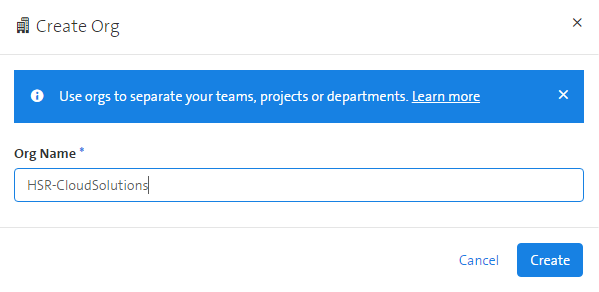
\includegraphics[width=0.65\columnwidth, valign=T]{images/swisscom_create_space/1.png}
 \\ \hline
Als Space Name wählen wir ddd (Name der App).
&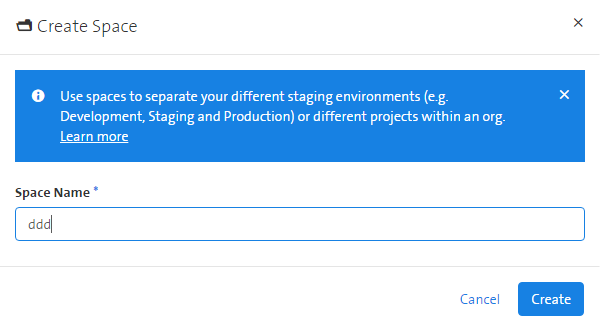
\includegraphics[width=0.65\columnwidth, valign=T]{images/swisscom_create_space/2.png}
 \\ \hline
In Eclipse muss ein neuer Server erfasst werden. Anstatt Tomcat verwenden wir nun einen Cloud Foundry Server
&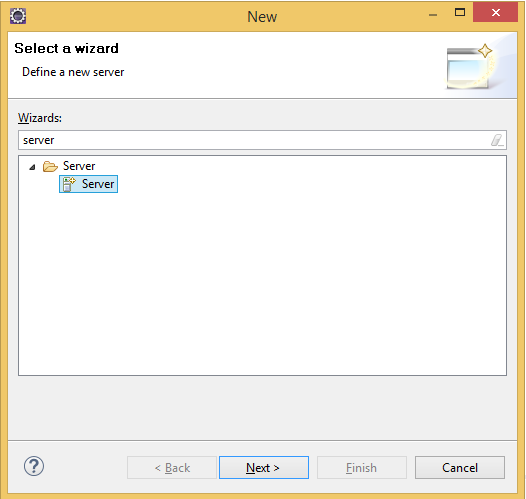
\includegraphics[width=0.65\columnwidth, valign=T]{images/ddd_cloud_deployment/1.png}
 \\ \hline 
Durch das zuvor im Marketplace installierte Plugin kann nun ein Cloud Foundry Server ausgewählt werden.
&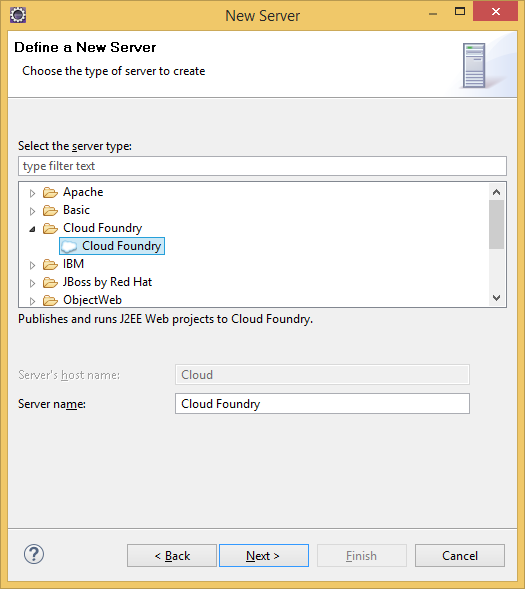
\includegraphics[width=0.65\columnwidth, valign=T]{images/ddd_cloud_deployment/2.png}
 \\ \hline
Die Logindaten des Swisscom Application Cloud Accounts müssen hier hinterlegt werden. Die URL \glqq https://api.lyra-836.appcloud.swisscom.com\grqq  muss erfasst werden.
&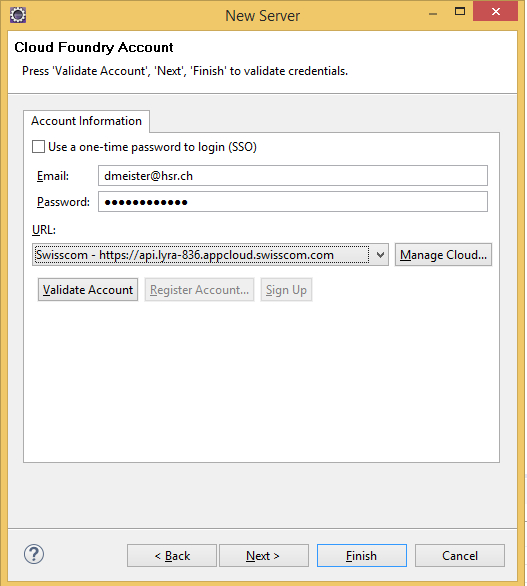
\includegraphics[width=0.65\columnwidth, valign=T]{images/ddd_cloud_deployment/3.png}
 \\ \hline
Die zuvor erstellte Org und Space sollten nun erscheinen. Den gewünschten Space auswählen um fortzufahren.
&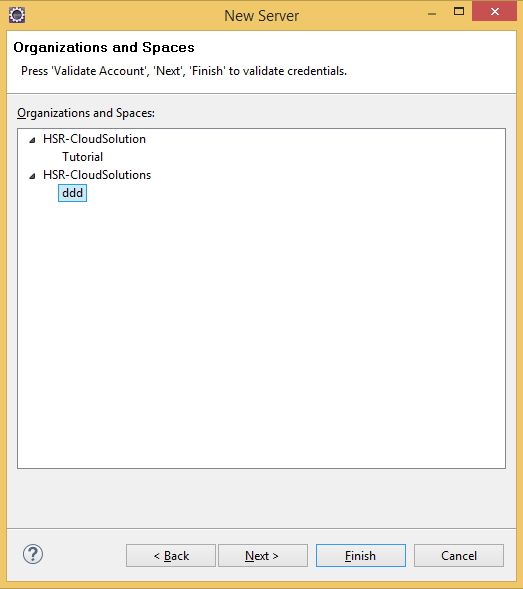
\includegraphics[width=0.65\columnwidth, valign=T]{images/ddd_cloud_deployment/4.png}
 \\ \hline 
Den App Namen kann man belassen oder falls gewünscht anpassen.
&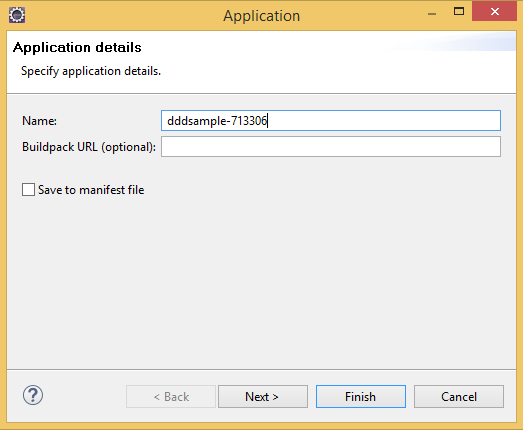
\includegraphics[width=0.65\columnwidth, valign=T]{images/ddd_cloud_deployment/5.png}
 \\ \hline
Falls benötigt kann das Memory Limit erhöht werden.
&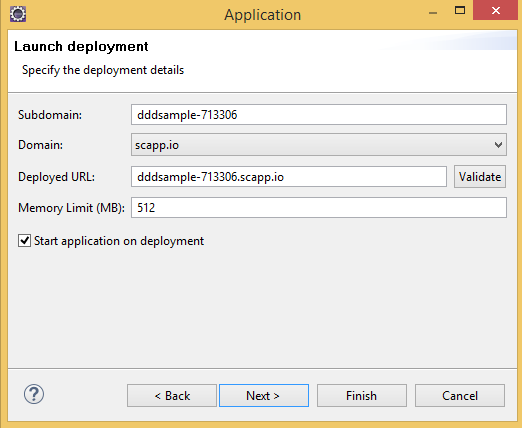
\includegraphics[width=0.65\columnwidth, valign=T]{images/ddd_cloud_deployment/6.png}
 \\ \hline
Nun startet der Deployment Prozess, nach kurzer Zeit ist er erfolgreich abgeschlossen.
&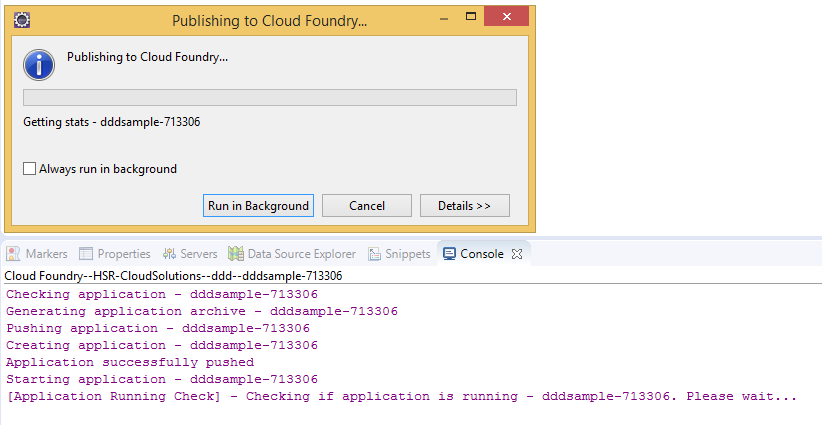
\includegraphics[width=0.65\columnwidth, valign=T]{images/ddd_cloud_deployment/7.png}
 \\ \hline
Auf der Application Cloud Console erscheint nun die laufende App.
&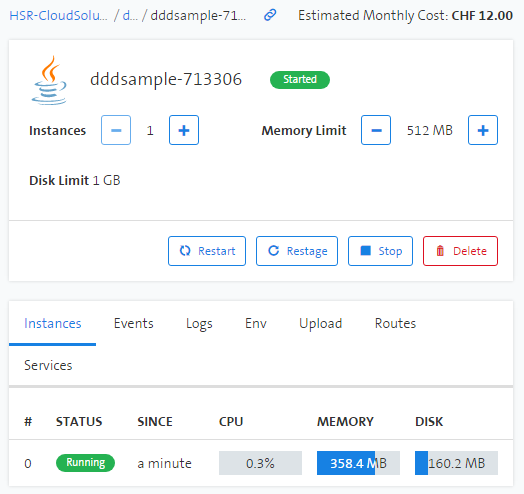
\includegraphics[width=0.65\columnwidth, valign=T]{images/ddd_cloud_deployment/8.png}
 \\ \hline
\end{longtable}
\section{Fazit}
Der grundlegende Teil dieser Aufgabe war mit der Swisscom Application Cloud sehr angenehm zu lösen. Durch die Online-Dokumentation wird man gut durch das Deployment durchgeführt. Die Applikation selbst, respektive der Code musste nicht angepasst werden. 

Anfangs hatten wir der Ausführung von gewissen Funktionen. Es stellte sich schnell heraus, dass wir vergessen haben, die Maven Dependencies zu laden und das Projekt zu builden.
\chapter{Hands-On: Erweiterung um relationale Datenbank}
Die DDD Sample App arbeitet standardmässig mit HyperSQL DB (HSQLDB). Dies ist in der Datei jdbc.properties unter /src/main/resources ersichtlich. 

Die Swisscom Application Cloud bietet keinen MySQL Service. Stattdessen wird MariaDB als vertreter relationaler Datenbank angeboten. 

\begin{longtable}{| p{5cm} | p{11cm} |}
\hline
MariaDB muss auf dem zuvor erstellten Space (ddd) hinzugefügt werden. Für diese Aufgabe reicht die kleinste Variante mit 1GB Storage und 10 Connections.
&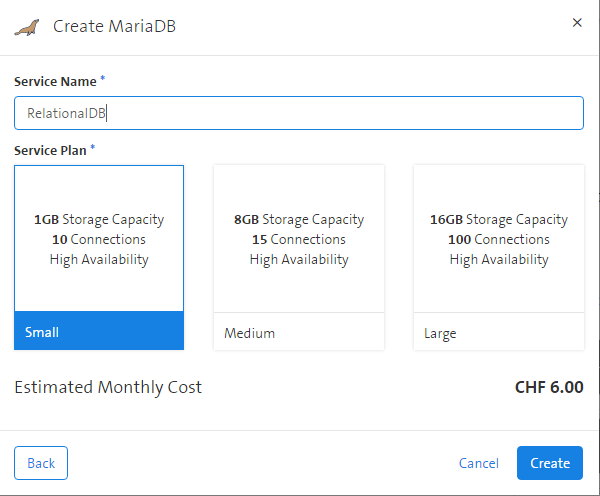
\includegraphics[width=0.65\columnwidth, valign=T]{images/mariadb/1.png}
 \\ \hline
Sobald erstellt, müssen im Reiter \glqq Serivce Keys \grqq noch Zugriffsschlüssel erstellt werden. Diese müssen dann in der verwendeten App zur Authentifizierung hinterlegt werden.
&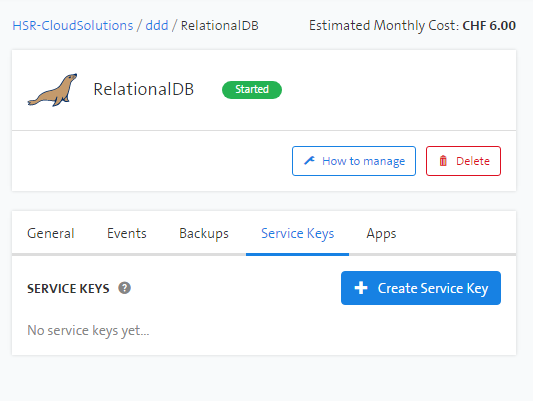
\includegraphics[width=0.65\columnwidth, valign=T]{images/mariadb/2.png}
 \\ \hline
Den Keys kann ein beliebiger Name hinterlegt werden.
&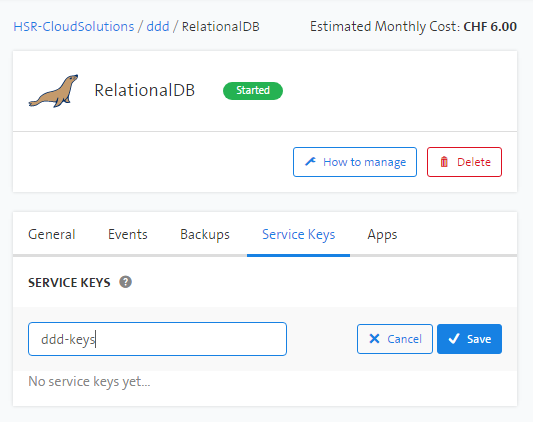
\includegraphics[width=0.65\columnwidth, valign=T]{images/mariadb/3.png}
 \\ \hline 
Die benötigten Informationen liegen nun im JSON Format da. Die private IPv4 Addresse im host-Feld verrät, dass ein externer Zugriff ausserhalb der Swisscom Application Cloud nicht möglich ist. Sowohl Username und Passwort sind ein zufällig generierter String.
&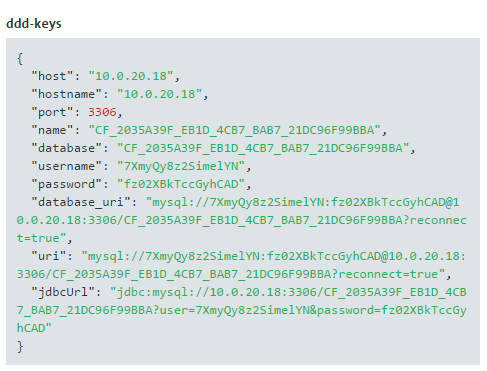
\includegraphics[width=0.65\columnwidth, valign=T]{images/mariadb/4.png}
 \\ \hline
Der bestehenden App kann nun der zuvor erstellte DB Service gebunden werden.
&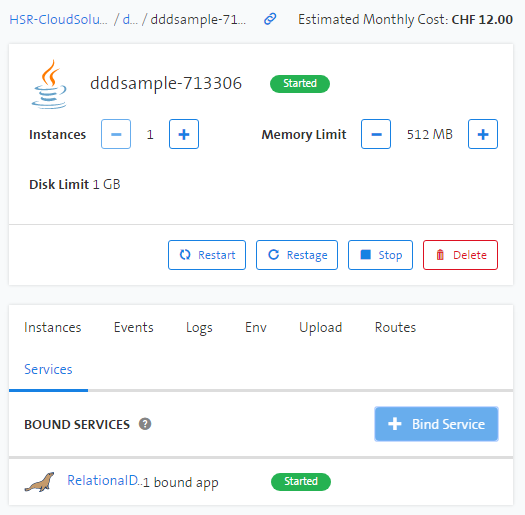
\includegraphics[width=0.65\columnwidth, valign=T]{images/mariadb/5.png}
\\ \hline 
Wir benötigen für die App nun die MariaDB Dependencies, welche wir einfach mit Maven hinzufügen können. Wir verwenden die als funktionierend empfohlene Version 1.1.7.
&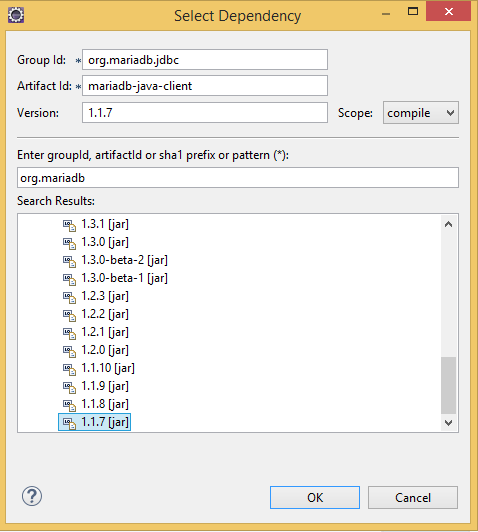
\includegraphics[width=0.65\columnwidth, valign=T]{images/mariadb/6.png}
\\ \hline 
Damit die Änderungen in der Datenbank auch nach dem Neustart persistent sind, müssen wir eine Anpassung der Konfiguration im File hibernate.properties vornehmen. Im Feld hibernate.hbm2ddl.auto müssen wir die Einstellung von \glqq create drop\grqq (nicht persistent) nach \glqq update\grqq ändern. 
&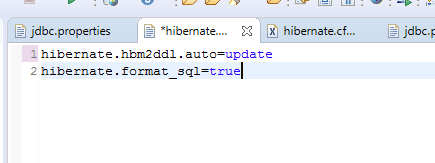
\includegraphics[width=0.65\columnwidth, valign=T]{images/mariadb/7.png}
\\ \hline 
Nun muss nur noch im File jdbc.properties der zu verwendende Treiber und der Connection String angepasst werden.
&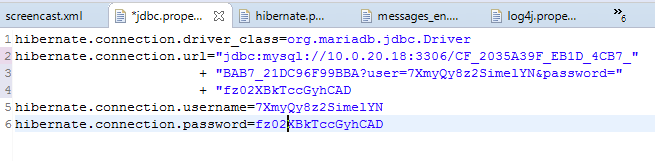
\includegraphics[width=0.65\columnwidth, valign=T]{images/mariadb/8.png}
\\ \hline 
\end{longtable}

Die Änderungen müssen nun mit Maven Update, resp. Maven Build angepasst und neu gepusht werden.

\section{Security Überlegungen}
Die Datenbankservices sind bei Swisscom nur über IP Adressen aus dem privaten Adressbereich erreichbar. Dies lässt schliessen, dass Swisscom selbst in ihrem Datacenter die Datenbanken hostet. Eine direkte Anbindung der Datenbank ausserhalb der Swisscom App Cloud ist daher nicht möglich. 

Die Zugriffe zur Datenbank sind mittels zufallsgenerierten Strings für Username und Passworte authentisiert. Eine TLS verschlüsselte Verbindung zwischen App und Datenbank wäre ebenfalls wünschenswert und im Falle eines Zugriffs aus dem Internet (hier nicht der Fall) zwingend notwendig. Wir haben leider keine Informationen betreffend Verschlüsselung der Verbindungen gefunden, und ein Sniffen des Netzwerkverkehrs ist für uns leider nicht ohne weiteres Möglich. 

\section{Fazit}
Die Anbindung der MariaDB ist sehr einfach. In der Applikation muss nur der zu verwendende Connection String angepasst werden. Das Erstellen des Services und der Keys ist einfach und scheint gelungen. Einzig, dass keine Informationen betreffend Verschlüsselung vorhanden sind, ist nicht optimal.

Wir hatten keine gröberen Probleme, haben aber festgestellt, dass nach dem Starten der App noch etwas gewartet werden muss, ansonsten kann die App abstürzen. Dies liegt wohl an längeren Ladezeiten im Hintergrund. 

Die Dokumentation musste nicht konsultiert werden. Die Erstellung des Services ist sehr einfach und benötigt keine Erklärungen. In der DDD App mussten wir die zu verändernden Files kurz suchen, im Grossen und Ganzen hatten wir aber wenig Probleme.

\section{Weitere Storage Offerings}
Mit MariaDB und MongoDB werden die Storage Offerings \glqq Relational Database\grqq und \glqq Key-Value Storage\grqq gemäss Cloud Computing Patterns (CCP) angeboten. Als in Memory-Store, welcher ebenfalls dem CCP \glqq Key-Value Storage\grqq zugeordnet werden kann, wird Redis angeboten. Als Speicher für grosse Datasets bietet Swisscom den \glqq S3 Dynamic Storage\grqq . Dieser Service ist dem CCP \glqq Blob Storage\grqq zuzuordnen.

\chapter{Hands-On: NoSQL-Persistence in der Cloud (am Beispiel MongoDB)} %DONE
\section{Anleitung}
Für diese Aufgabe wurde das ContractManagement verwendet. Dieses bereitete aber keine grossen Probleme.
\begin{longtable}{| p{5cm} | p{11cm} |}
\hline
Auf der PaaS Platform der Swisscom kann man sehr einfach einen neuen Service hinzufügen. Dazu wählt man nur Create Service und klickt auf MongoDB. &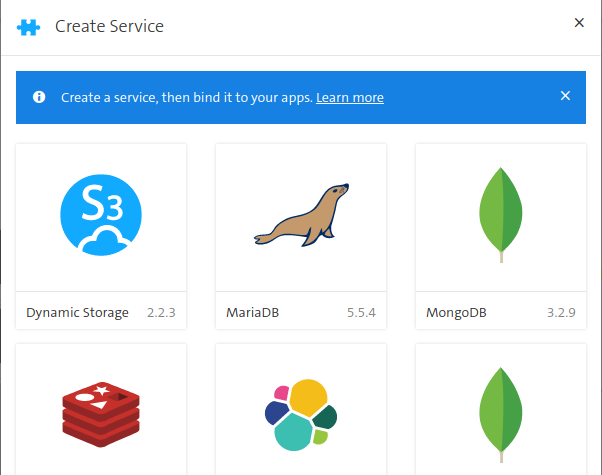
\includegraphics[width=0.65\columnwidth, valign=T]{images/mongodbexample/image1.png}
 \\ \hline
 Nun vergibt man einen Namen und wählt die gewünschte Grösse. Für dieses kleine Projekt reicht Small vollkommen aus.
&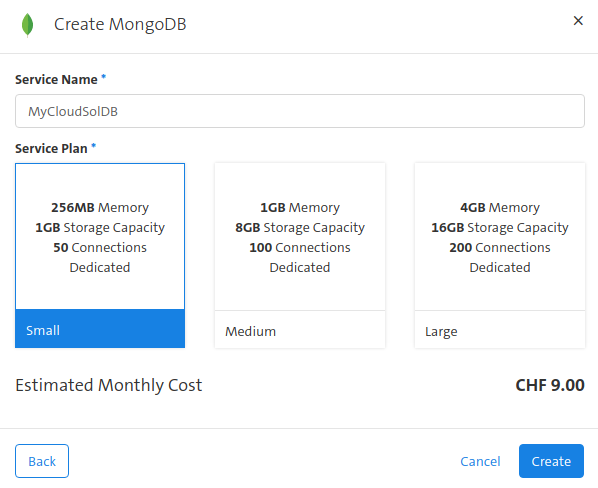
\includegraphics[width=0.4\columnwidth, valign=T]{images/mongodbexample/image2.png}
 \\ \hline
Dies erstellt automatisch die neue MongoDB. Nach ca. 1-2 Minuten ist diese bereit und kann konfiguriert werden. Damit man eine Verbindung zur Datenbank herstellen kann, muss man einen Service Key erstellen. Dies geschieht durch einen klick auf Create Service Key.
&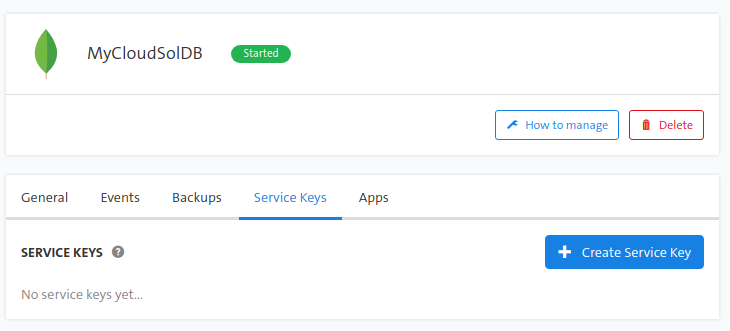
\includegraphics[width=0.65\columnwidth, valign=T]{images/mongodbexample/image3.png}
 \\ \hline
Für den Service Key gibt man einen passenden Namen und klickt auf Save.
&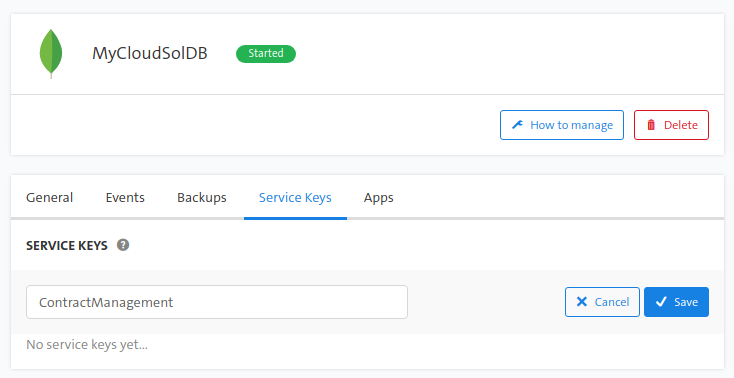
\includegraphics[width=0.65\columnwidth, valign=T]{images/mongodbexample/image4.png}
 \\ \hline
Nun erhält man die Zugangsdaten und kann diese kopieren...
&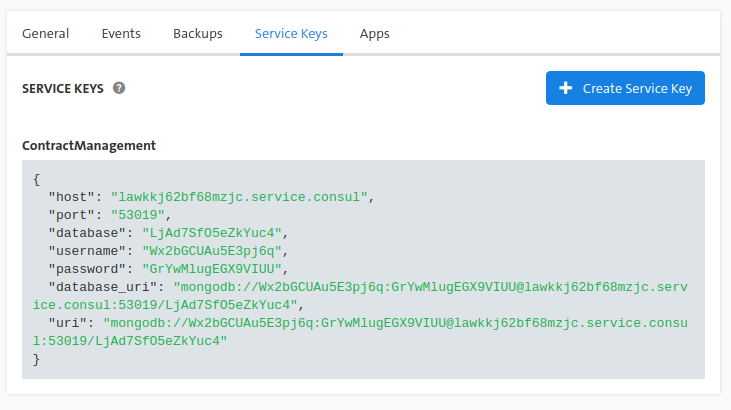
\includegraphics[width=0.65\columnwidth, valign=T]{images/mongodbexample/image5.png}
 \\ \hline
... und in der Applikation hinterlegen. Nun funktioniert die Verbindung zur MongoDB und man muss die Applikation wie bei Aufgabe 1 auf die Plattform laden.&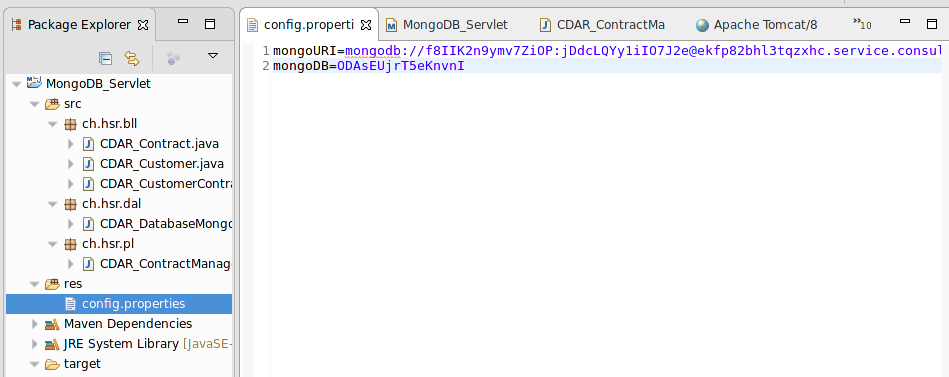
\includegraphics[width=0.65\columnwidth, valign=T]{images/mongodbexample/image6.png}
 \\ \hline
\end{longtable}

\section{Fragen}
\subsection{Was has wie erwartete funktioniert?}
Eigentlich hat alles wie geplant funktioniert. Einzig bei Eclipse hatten wir zuerst Probleme, da wir es zuerst Local mit Tomcat starten wollten, was aber nicht funktionierte. Doch mit dem Hochladen hat die Applikation sofort funktioniert. Grössere Konfigurationen mussten nicht gemacht werden.
\subsection{Was hat nicht funktioniert?}
Nichts. Alles hat ohne Probleme funktioniert. 
\subsection{Wie schätzen Sie die Sicherheit dieses Datenbank-Hostings ein?}
Die Datenbank befindet sich für alle Erreichbar im Internet. Abgesichert wird die Datenbank lediglich durch ein Passwort und einen Benutzernamen. Diesen kann man aber nicht selber bestimmen oder abändern, was nicht sehr praktisch ist., Auch der Datenbankname kann nicht selber bestimmt oder angepasst werden. Es wird ein zufälliger Namen generiert. 


\chapter{Analyse: Service Level Agreements(SLAs)} %DONE
\section{Fragen}
\subsection{Gibt es ein oder mehrere Service Level Objectives (SLOs)?}
Bei der Swisscom gibt es mehrere Service Level Objectives. Es wird in verschiedene Kategorien unterteilt, wie zum Beispiel Availability, Security oder Continuity. Dabei wird jeder Punkt nochmals in drei SLA Stufen unterteilt. Diese sind Standard Public, Standard Virtual Private und Premium Virtual Private. So sind alle SLOs sehr genau beschrieben. Leider bietet die Swisscom momentan aber nur Best Effort an. Die SLAs sind für spätere Releases geplant, stehen aber schon bereit. Genauere angaben, ab wann diese gelten, konnten nicht gefunden werden. 
\subsection{Questions to Ask}
\subsubsection{How are uptime and availability calculated?}
Diese Angabe ist bei der Swisscom vorhanden und wird wie folgt beschrieben:
\begin{quote}
The availability of each of the marketplace cloud services are measured by transactions on a reference service
instance on the production. If these measurements show, that service is running, the availability status
is set to „available” for this service. Unless otherwise stated, availability of the reference service is
checked every 60 seconds and if two subsequent checks are failing the service is considered as unavailable.
\end{quote}
Dabei wird nicht zwischen Uptime und Availability unterschieden.
\subsubsection{What should be in place for me to be covered?}
Die Swisscom unterscheidet zwischen ''Normal Availability'' und ''High Availability''. Normal Availability bedeutet das man nur eine Instanz gestartet hat. High Availability bedeutet ein Cluster von Nodes. Das heisst mindestens zwei Nodes müssen gestartet sein. Zwischen Normal und High Availability liegen je nach Bezahlmodel 0.3 oder 0.4 Prozent Verfügbarkeit.
\subsubsection{What about performance degradation as opposed to hard downtime?}
Es werden zwei verschiedene SLAs angegeben. Der erste ist für die Instanz, sowie für das Cloud Management. Der zweite ist für den Marketplace Cloud Services. Beide enthalten untschiedliche SLOs, welche wieder in die verschiedenen Bezahlmodelle unterteilt sind.
\subsubsection{What are the penalties for SLA violations?}
Zu diesem Bereich gibt es keine genaueren Angaben. Im Dokument ist dazu nichts zu finden und man muss sich wahrscheinlich bei der Swisscom melden. Ob und wie man ausgezahlt wird, war auch nicht auffindbar.
\subsubsection{What do I have to do to request a credit?}
Wie bereits in der vorherigen Frage geschrieben, findet man zu diesem Thema nicht wirklich eine Angabe.
\subsection{Fehlen bestimmte Evaluationskriterien?}
Bei dem White Paper von Dimension Data geht es Hauptsächlich um Uptime und Availability. Heutzutage sollte man auch immer an das Thema Security denken. Dies wird viel zu häufig vernachlässigt. Der Rest deckt aber sehr viel ab und ist gut als Evaluationshilfe geeignet. 
\subsection{Ist die Einhaltung und Existenz von SLAs wichtig?}
\textbf{a)}
Bei der Entscheidung ob man sein Produkt in die Cloud verlagert, sind die SLAs enorm wichtig. Diese Vergleicht man meistens mit seinen eigenen Möglichkeit. Zum Beispiel die Verfügbarkeit kann man dies einfach vergleichen. Möchte man eine hochverfügbare Umgebung aufbauen, oder ist eine fremde Cloud kostengünstiger. Dabei verlässt man sich immer auf die SLAs und möchte auch mit dieser rechnen können. 
\textbf{b)}
Auch bei der Wahl des Providers sind die SLAs enorm wichtig. Es gibt immer wie mehr Cloudanbieter und ohne SLAs kann man diese kaum miteinander vergleichen. Auch das einhalten ist wichtig, besonders für den Anbieter. Denn sobald die SLAs mehrmals gebrochen wurden, hat der Anbieter mit Kundenverlust zu rechnen.
\subsection{Weitere wichtige Dokumente}
\href{"https://developer.swisscom.com/terms/SLADefinitions-en.pdf"}{SLA-Definitions - Enterprise Customers}\\
\href{"https://www.swisscom.ch/content/dam/swisscom/de/biz/sme/mykmuoffice/pdf/SLA_Besondere_Bedingungen_dt.pdf"}{Besondere Bedienungen}

\chapter{Konzept: Cloud Computing Patterns (CCP)}
Bei der Swisscom wird für die PaaS-Umgebung die Lösung von Cloud Foundry eingesetzt. Die Architektur sieht folgendermassen aus:
\begin{figure}[H]
\centering
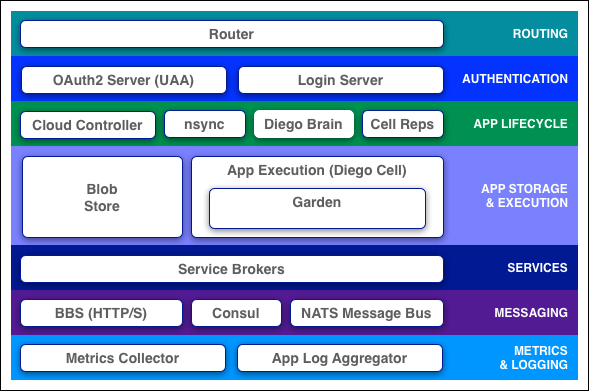
\includegraphics[scale=0.45]{images/ccp/cloudfoundry.png}
\caption{Cloud Foundry Architektur}
\end{figure}
Zum Vergleich ist hier nochmals das Standardarchitektur Pattern:
\section{Abbildung auf das CCP Architecture Overview Diagram}
\begin{figure}[H]
\centering
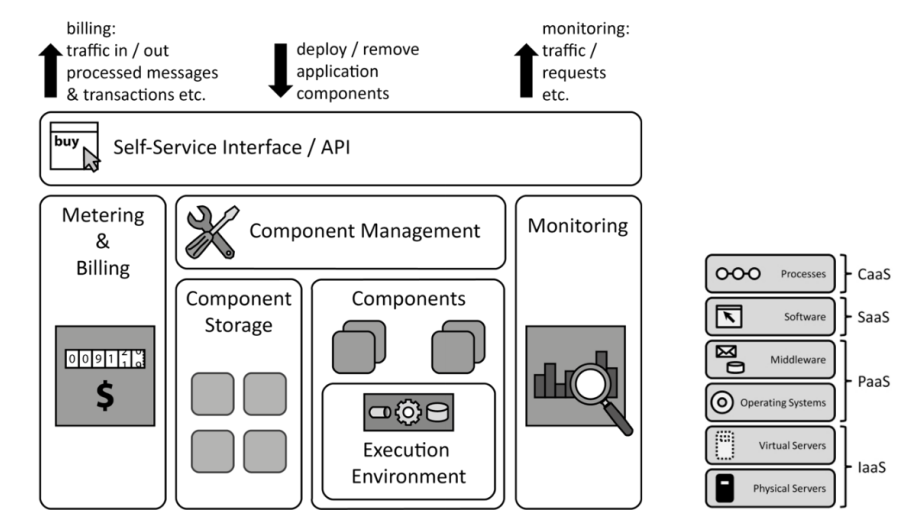
\includegraphics[scale=0.4]{images/ccp/ccp.png}
\caption{CCP Architektur Diagramm}
\end{figure}
\subsection{Mappingtabelle}
\begin{table}[H]
\begin{tabular}{|c|c|}
\hline 
\textbf{CCP Architecture Overview Diagram} & \textbf{Swisscom - Cloud Foundry} \\ 
\hline 
Self-Service Interface / API & Router, Login Server / UAA \\ 
\hline 
Metering und Billing & Metrics Collector, App Log Aggregator \\ 
\hline 
Component Management & Cloud Controller \\ 
\hline 
Monitoring & Health Manager \\ 
\hline 
Component Storage & Blob Store \\ 
\hline 
Components & Warden \\ 
\hline 
Execution Enviroment & Application Execution (DEA) \\ 
\hline 
\end{tabular} 
\end{table}

\section{Cloud-Deployment Modellierung}

\subsection{Fragen}
\subsubsection{Ist eine Decomposition-Strategie erkennbar?}
\subsubsection{Wir würden Sie die Applikation refactoren?}
Die Applikation müsste noch besser voneinander getrennt werden. Alle Komponenten sollte loser gestaltet sein, damit jeder Teil separat Überwacht und skaliert werden könnte. So würde die Applikation noch viel mehr von einer Cloud-Umgebung profitieren. Der Einsatz von Load-Balancer wäre so durchaus möglich. Oder auch andere Operation Management Pattern könnten viel einfacher Umgesetzt werden.

\subsubsection{Welches Workload Pattern liegt vor?}
Bei der Applikation ist das Unpredictable Workload Pattern erkennbar. Da es sich um ein Managementsystem handelt, kann man nicht vorhersagen, wann ein Benutzer die Applikation nutzt. Würde es fixe Wartungs- und Managementfenster geben, könnte die Last vorhergesagt werden. Aber sonst ist dies sehr schwer. Man weiss nur, dass die Last zu Arbeitszeiten sicher viel höher ist, denn um diese Zeit wird die Applikation eingesetzt.
\subsubsection{Wie sind Application State Management und Session State Management gelöst?}
Das Application State Management ...

Das Session State Management wird nach dem Pattern Stateless Component umgesetzt. Alle Anfragen werden ohne State an die Applikation gesendet und werden verarbeitet. 

\subsubsection{Welche Cloud Computing Patterns aus der Rubrik Cloud Application Components sehen Sie?}


\subsubsection{Sollte Ihrer Meinung nach das Watchdog Pattern implementiert werden?}
Nein, dies sollte nicht implementiert werden. Bevor dies möglich wäre, müsste man die Applikation zuerst noch umbauen. Die einzelnen Komponenten sind zu sehr Miteinander verbunden, um sie separat Überwachen zu können. Einzig der LwM2M Server könnte man überwachen und bei Fehlern sofort wieder Neustarten, da dieser separat von dem Rest der Applikation läuft. Aber auch für dies muss der Server noch umgebaut werden, damit die Applikation die Anfragen in einer Queue zwischenspeichern kann, damit beim Starten des neuen Servers keine Probleme entstehen.
\chapter{Analyse: SWOT-Assessment von Cloud Provider und Cloud Offering}
\begin{table}[H]
\begin{tabular}{|l|p{0.4\textwidth}|p{0.4\textwidth}|}
\hline 
 & \textbf{Positiv (Nützlich)}  & \textbf{Negativ (Schädlich)} \\ \hline 
\textbf{Interne} & \textbf{Stärken} 
\begin{itemize}
\item Schweizer Datenschutzgesetz
\item Grosse Produktvielfalt
\item Markenansehen in der Schweiz
\item Grosse Community mit Cloud Foundry
\end{itemize}

& \textbf{Schwächen}
\begin{itemize}
\item Viele Ausfälle
\item Teurer als Konkurrenten
\item Hohe Entwicklungskosten
\end{itemize}
\\ \hline 
\textbf{Externe} & \textbf{Chancen} 
\begin{itemize}
\item Ausbau im europäischen Markt
\item Unterstützung der Cloud Foundry (Open Source)
\end{itemize}&
\textbf{Bedrohungen (Risiken)} 
 \begin{itemize}
\item Kundenverlust durch Ausfälle
\item Extrem viele und grosse Konkurrenten
\end{itemize}
\\ \hline 
\end{tabular} 
\end{table}

\chapter{Konzept: Provider Evaluation Checkliste}
\begin{table}[H]
\begin{tabular}{|p{0.3\textwidth}|l|p{0.5\textwidth}|}
\hline 
 & Erfüllt? & Kommentar \\ 
\hline 
Kriterium 1 & Ja & • \\ 
\hline 
Kriterium 2 & Nein & • \\ 
\hline 
Kriterium 3 & • & • \\ 
\hline 
Kriterium 4 & • & • \\ 
\hline 
Kriterium 5 & • & • \\ 
\hline 
Kriterium 6 & • & • \\ 
\hline 
Kriterium 7 & • & • \\ 
\hline 
Kriterium 8 & • & • \\ 
\hline 
Kriterium 9 & • & • \\ 
\hline 
Kriterium 10 & • & • \\ 
\hline 
\end{tabular} 
\end{table}

\chapter{Analyse: Management Summary}
Maximal 1 Seite

